%!TEX root = ../main.tex

\section{Discussion and Analysis}
\label{section:case-study}

Figure~\ref{fig:distances} shows the mean Manhattan distance of the perturbed examples in each iteration of FOCUS, along with the proportion of perturbations resulting in valid counterfactual examples found for two datasets (we omit the others due to space considerations). These trends are indicative of all settings: the mean distance increases until a counterfactual example has been found for every $x$, after which the mean distance starts to decrease. This seems to be a result of the hinge-loss in FOCUS, which first prioritizes finding a valid counterfactual example (see Equation~\ref{eq:cfexample}), then decreasing the distance between $x$ and $\bar{x}$. 

\begin{figure}[t]
\begin{center}
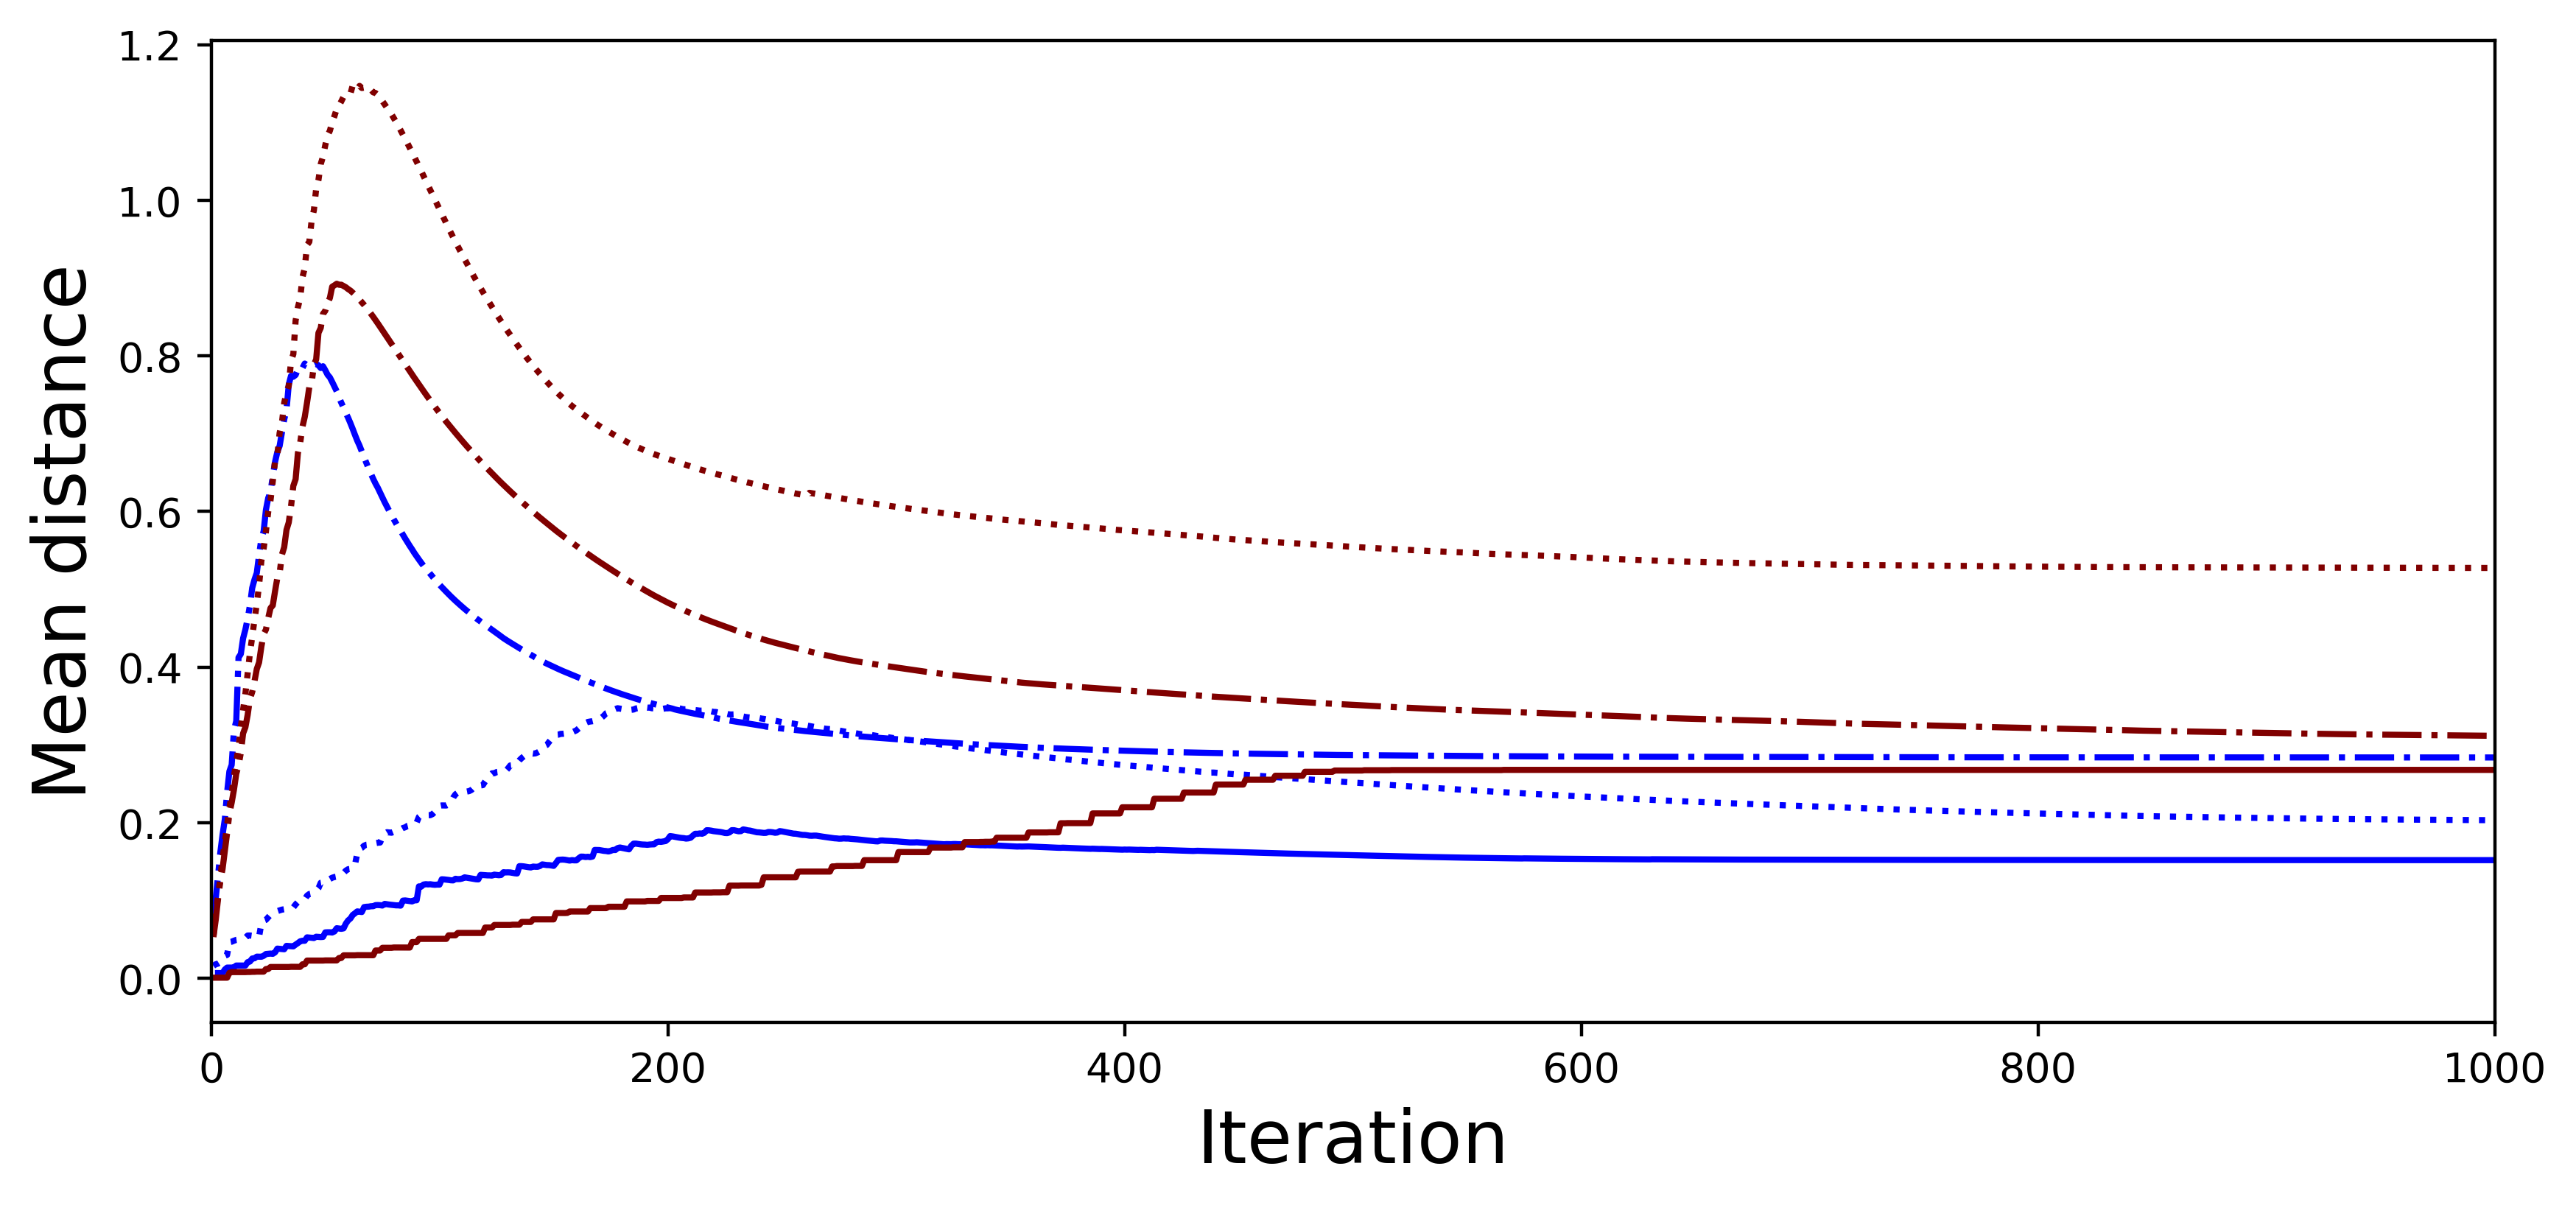
\includegraphics[scale=0.45]{04-research-focus/figures/mean_dist_manhattan_heloc_wine} 
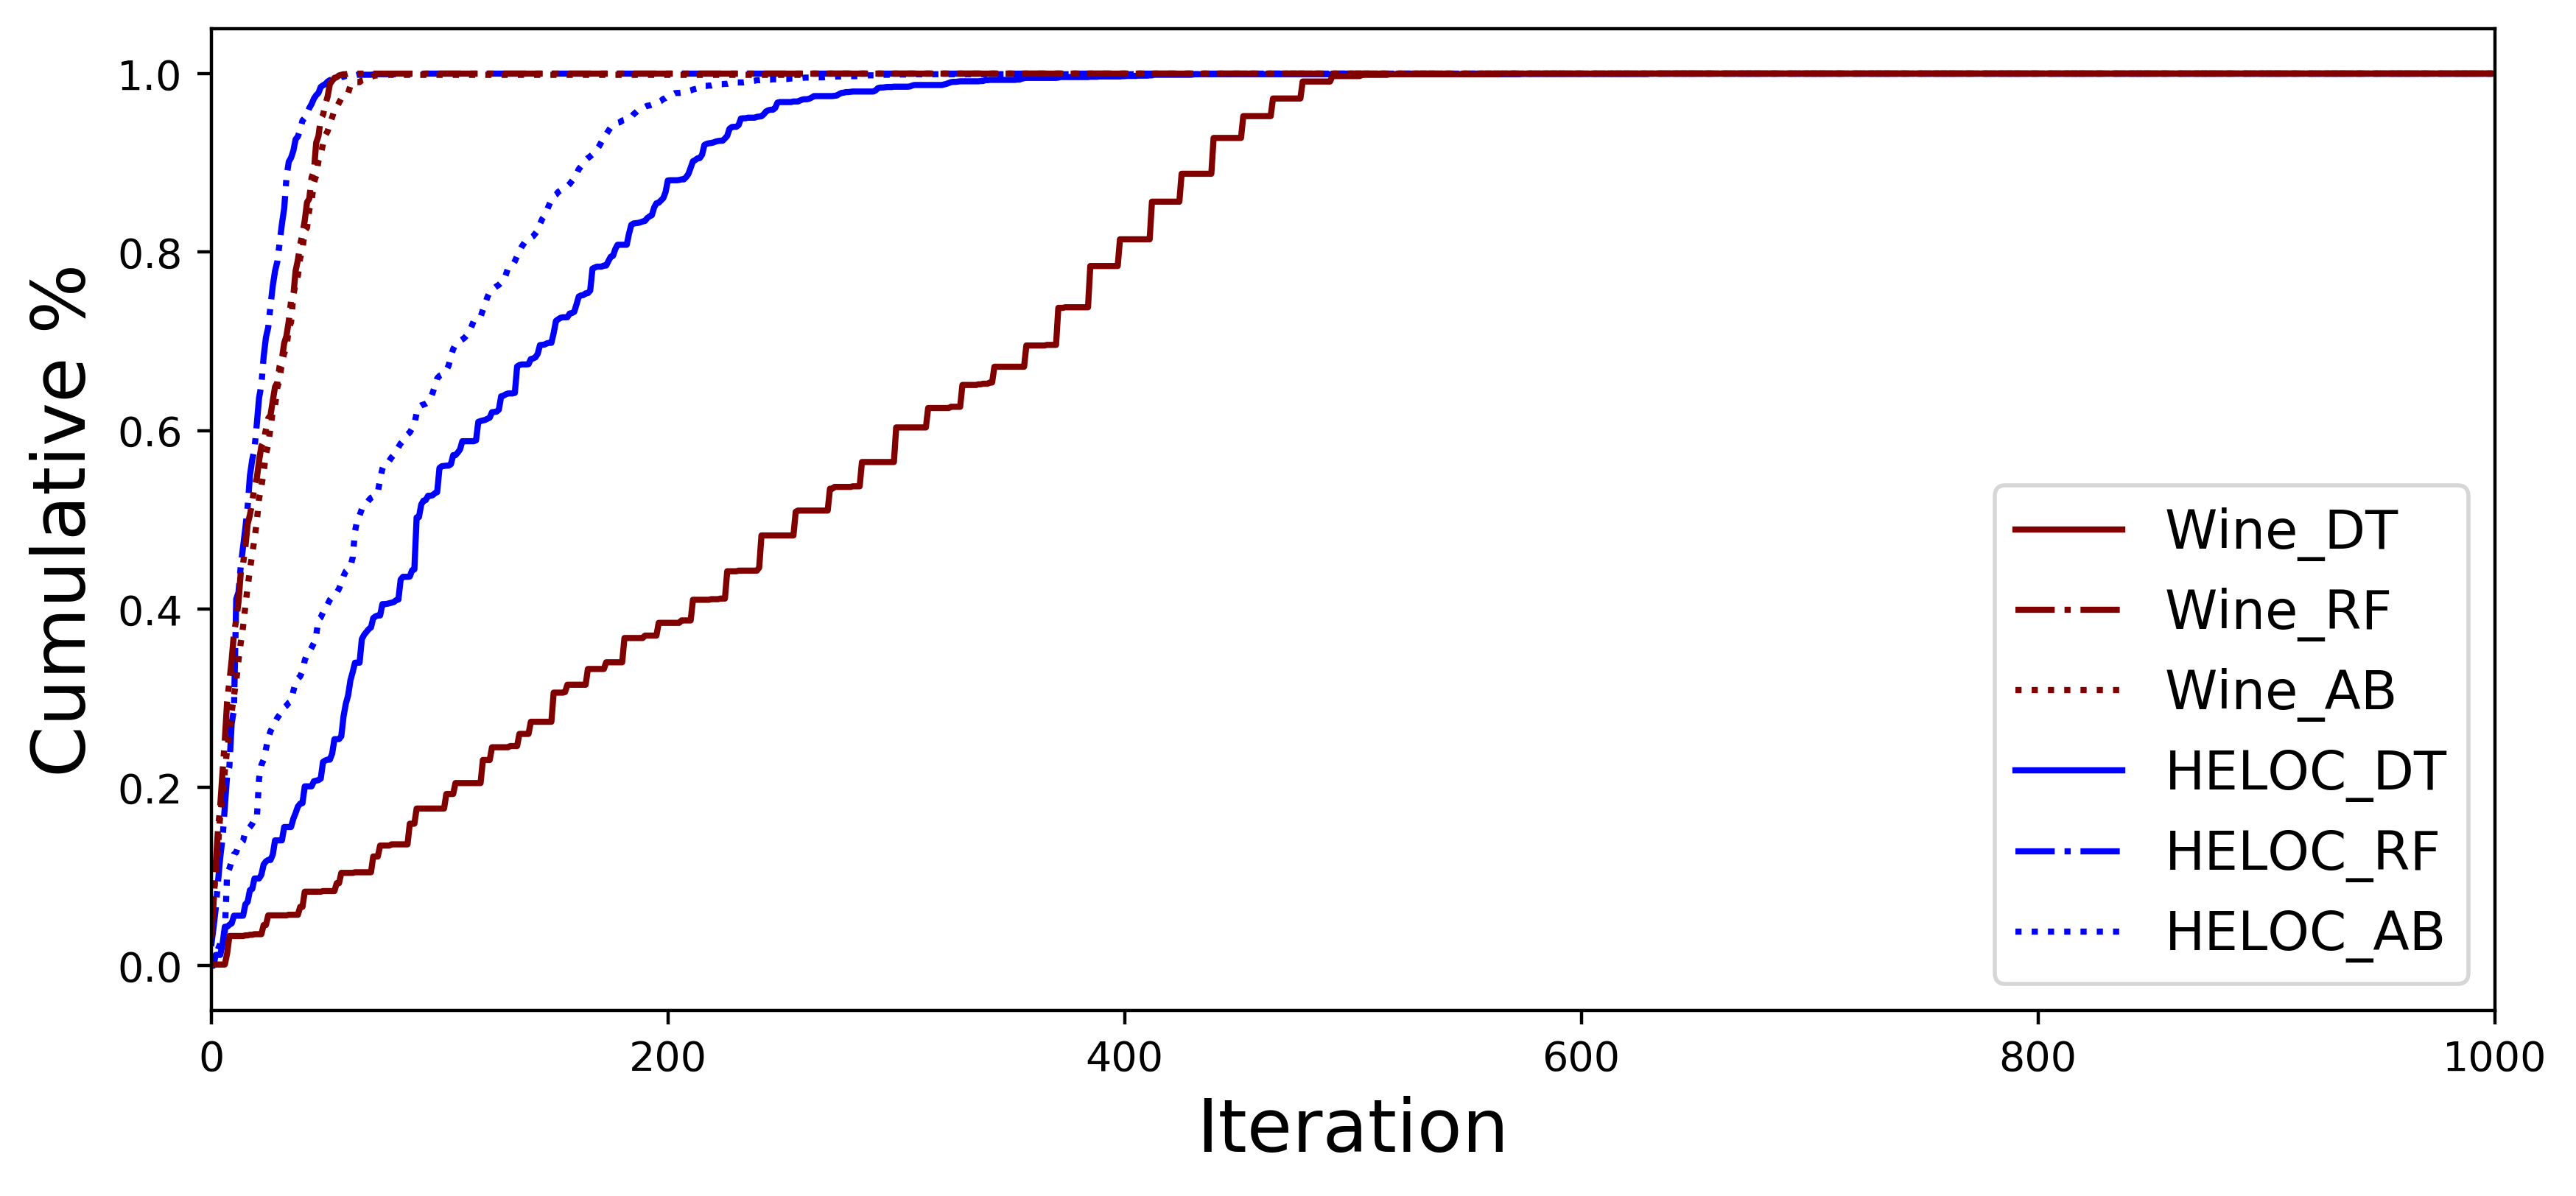
\includegraphics[scale=0.45]{04-research-focus/figures/iter_manhattan_heloc_wine} 
\end{center}
\caption{Mean distance (top) and cumulative \% (bottom) of counterfactual examples in each iteration of FOCUS for Manhattan explanations.}
\label{fig:distances}
\end{figure}



\begin{figure*}[h!]
\centering
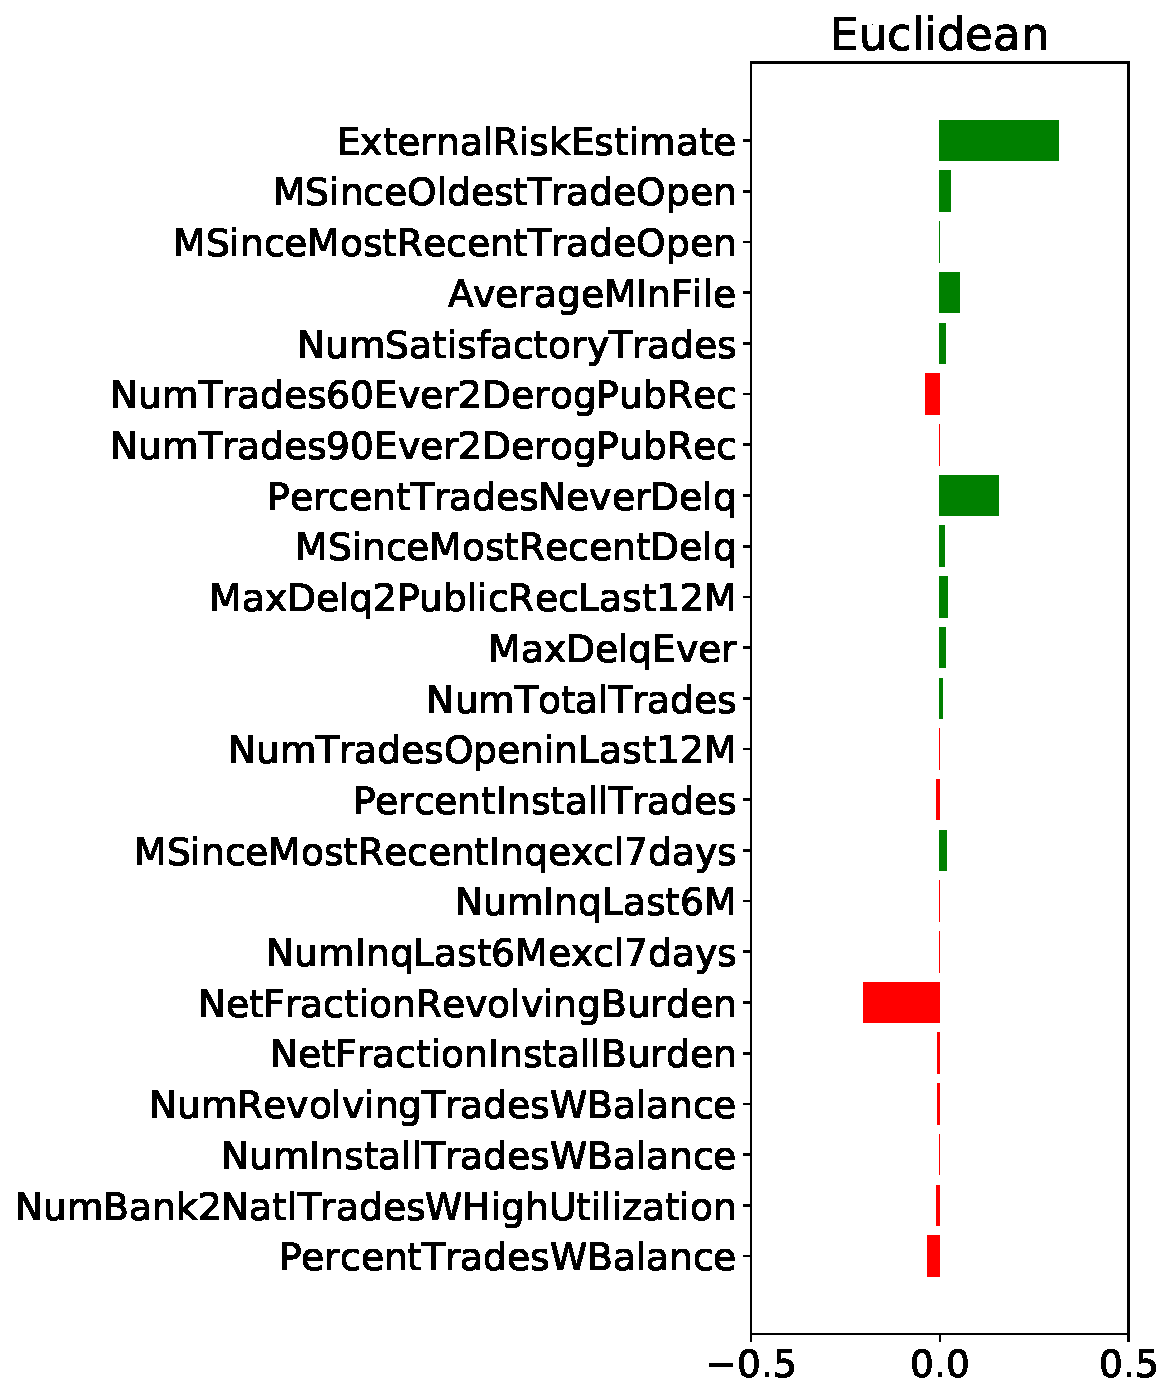
\includegraphics[scale=0.26]{04-research-focus/figures/perturb_euclid_heloc.pdf}
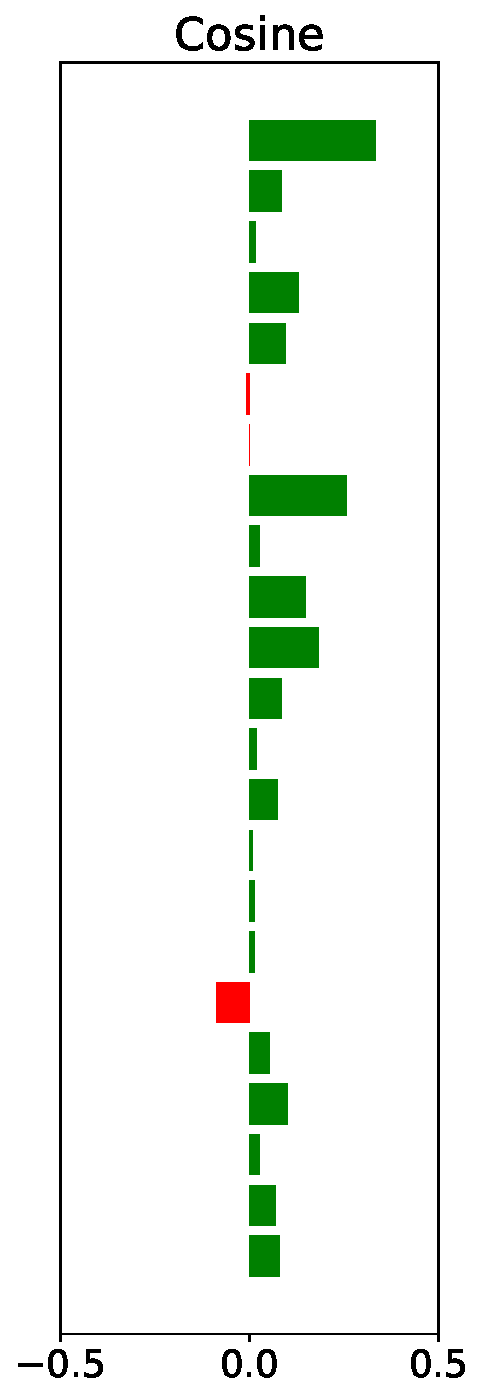
\includegraphics[scale=0.26]{04-research-focus/figures/perturb_cosine_heloc.pdf} 
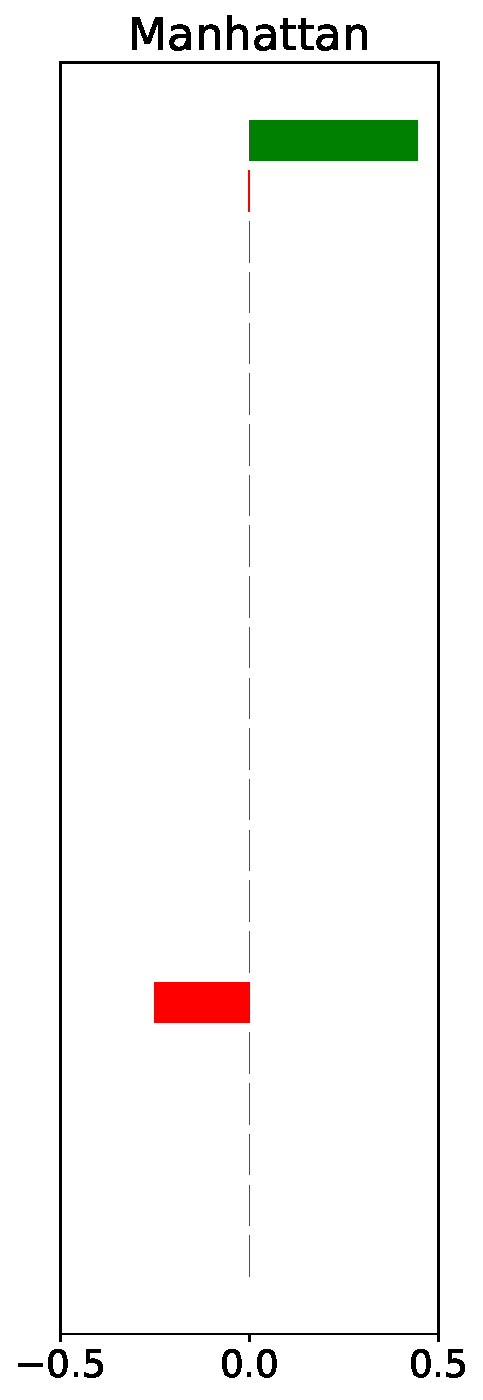
\includegraphics[scale=0.26]{04-research-focus/figures/perturb_manhat_heloc.pdf} 
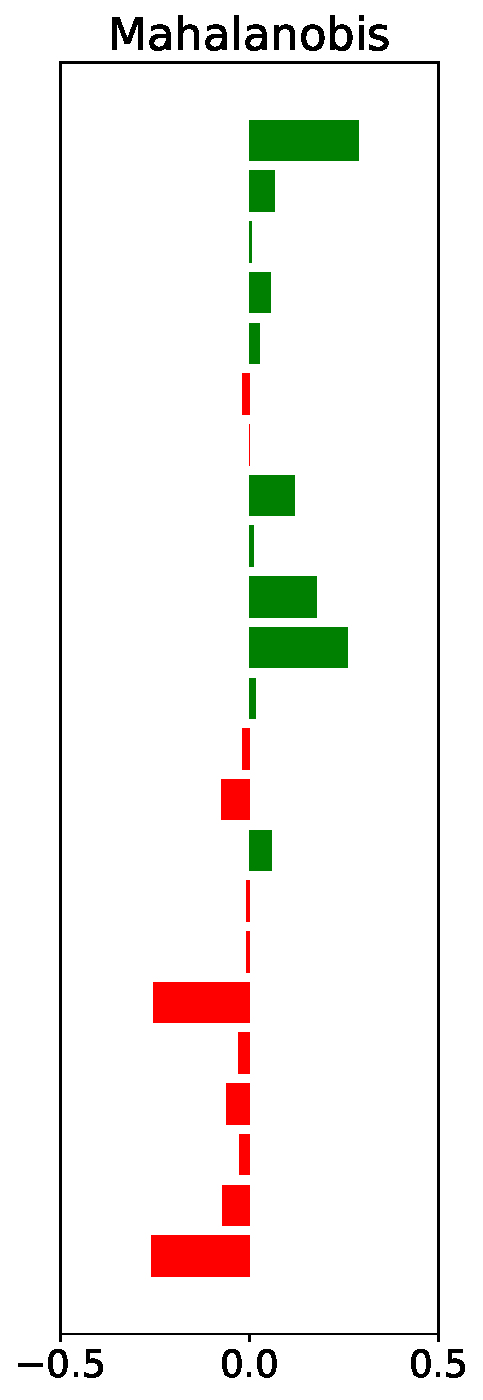
\includegraphics[scale=0.26]{04-research-focus/figures/perturb_mahal_heloc.pdf} 
\caption{FOCUS explanations for the same model and same $x$ from the \textsc{HELOC} dataset based on different distance functions. 
Green and red indicate increases and decreases in feature values, respectively. 
Perturbation values are based on normalized feature values. 
Left: Euclidean explanation perturbs several features, but only slightly. 
Middle Left: Cosine explanation perturbs almost all of the features. 
Middle Right: Manhattan explanation perturbs two features substantially.
Right: Mahalanobis explanation perturbs almost all of the features. 
}
\label{fig:perturb-examples}
\end{figure*}

\subsection{Case Study: Credit Risk}
As a practical example, we investigate what FOCUS explanations look like for individuals in the \textsc{HELOC} dataset. 
Here, the task is to predict whether or not an individual will default on their loan. 
This has consequences for loan approval: individuals who are predicted as defaulting will be denied a loan. 
For these individuals, we want to understand how they can change their profile such that they are approved. 
Given an individual who has been denied a loan from a bank, a counterfactual explanation could be:
\begin{quote}
\textit{Your loan application has been denied. In order to have your loan application approved, you need to 
\begin{inparaenum}[(i)]
	\item increase your ExternalRiskEstimate score by 62, and
	\item decrease your NetFractionRevolvingBurden by 58.
\end{inparaenum}}
\end{quote}

\noindent%
Figure~\ref{fig:perturb-examples} shows four counterfactual explanations generated using different distance functions for the same individual and same model. 
We see that the Manhattan explanation only requires a few changes to the individual's profile, but the changes are large.
In contrast, the individual changes in the Euclidean explanation are smaller but there are more of them. 
In settings where there are significant dependencies between features, the Cosine explanations may be preferred since they are based on perturbations that try to preserve the relationship between features. 
For instance, in the \textsc{Wine Quality} dataset, it would be difficult to change the amount of citric acid without affecting the pH level. 
The Mahalanobis explanations would be useful when it is important to take into account not only correlations between features, but also the training data distribution. 
This flexibility allows users to choose what kind of explanation is best suited for their problem. 

Different distance functions can result in different \emph{magnitudes} of feature perturbations as well as different \emph{directions}. For example, the Cosine explanation suggests increasing \textit{PercentTradesWBalance}, while the Mahalanobis explanations suggests decreasing it. 
This is because the loss space of the underlying RF model is highly non-convex, and therefore there is more than one way to obtain an alternative prediction. When using complex models such as tree ensembles, there are no monotonicity guarantees. In this case, both options result in valid counterfactual examples. 

We examine the Manhattan explanation in more detail. 
We see that FOCUS suggests two main changes: 
\begin{inparaenum}[(i)]
	\item increasing the \textit{ExternalRiskEstimate}, and 
	\item decreasing the \textit{NetFractionRevolvingBurden}. 
\end{inparaenum}
We obtain the definitions and expected trends from the data dictionary created by the authors of the dataset. 
The \emph{ExternalRiskEstimate} is a ``consolidated version of risk markers'' (i.e., a credit score). 
A higher score is better: as one's \emph{ExternalRiskEstimate} increases, the probability of default decreases. 
The \textit{NetFractionRevolvingBurden} is the ``revolving balance divided by the credit limit'' (i.e., utilization). 
A lower value is better: as one's \emph{NetFractionRevolvingBurden} increases, the probability of default increases. 
We find that the changes suggested by FOCUS are fairly consistent with the expected trends in the data dictionary, as opposed to suggesting nonsensical changes such as increasing one's utilization to decrease the probability of default. 


Decreasing one's utilization is heavily dependent on the specific situation: an individual who only supports themselves might have more control over their spending in comparison to someone who has multiple dependents. 
An individual can decrease their utilization in two ways: 
\begin{inparaenum}[(i)]
	\item decreasing their spending, or
	\item increasing their credit limit (or a combination of the two).
\end{inparaenum}
We can postulate that (i) is more ``actionable'' than (ii), since (ii) is usually a decision made by a financial institution. 
However, the degree to which an individual can actually change their spending habits is completely dependent on their specific situation: an individual who only supports themselves might have more control over their spending than someone who has multiple dependents. 
In either case, we argue that deciding what is (not) actionable is not a decision for the developer to make, but for the individual who is affected by the decision. 
Counterfactual examples should be used as part of a human-in-the-loop system and not as a final solution. 

The individual should know that utilization is an important component of the model, even if it is not necessarily ``actionable'' for them. 
We also note that it is unclear how exactly an individual would change their credit score without further insight into how the score was calculated (i.e., how the risk markers were consolidated).
It should be noted that this is not a shortcoming of FOCUS, but rather of using features that are uninterpretable on their own, such as credit scores.
Although FOCUS explanations cannot tell a user precisely how to increase their credit score, it is still important for the individual to know that their credit score is an important factor in determining their probability of getting a loan, as this empowers them to ask questions about how the score was calculated (i.e., how the risk markers were consolidated).


